%----------------------------------------------------------------------------------------
%	PACKAGES AND OTHER DOCUMENT CONFIGURATIONS
%----------------------------------------------------------------------------------------

\documentclass[a0,landscape]{a0poster}
\usepackage[paperwidth=93in, paperheight=36in, textwidth=87in, textheight=30in, scale=2]{geometry}

\usepackage{multicol} % This is so we can have multiple columns of text side-by-side
\columnsep=100pt % This is the amount of white space between the columns in the poster
\columnseprule=3pt % This is the thickness of the black line between the columns in the poster

\usepackage[svgnames]{xcolor} % Specify colors by their 'svgnames', for a full list of all colors available see here: http://www.latextemplates.com/svgnames-colors

\usepackage{times} % Use the times font
%\usepackage{palatino} % Uncomment to use the Palatino font

\usepackage{graphicx} % Required for including images
\graphicspath{{figures/}} % Location of the graphics files

\usepackage{multirow}
%Middle allignment in tables.
\usepackage{array}

\usepackage{booktabs} % Top and bottom rules for table
\usepackage[font=small,labelfont=bf]{caption} % Required for specifying captions to tables and figures
\usepackage{amsfonts, amsmath, amsthm, amssymb} % For math fonts, symbols and environments
\usepackage{wrapfig} % Allows wrapping text around tables and figures
\usepackage{natbib}
\usepackage{fancytikzposter}

\begin{document}

%----------------------------------------------------------------------------------------
%	POSTER HEADER 
%----------------------------------------------------------------------------------------

\begin{minipage}[b]{0.85\linewidth}
\VERYHuge \color{NavyBlue} \textbf{Modeling the Evolution of Mimicry} \color{Black}\\[0.5cm] % Title
\Huge \textbf{Mohiul Islam \& Peter Grogono}\\[0.5cm] % Author(s)
\Huge Engineering \& Computer Science, Concordia University\\[0.5cm] % University/organization
\huge \texttt{moh\_i@encs.concordia.ca \& grogono@cse.concordia.ca}\\
\end{minipage}
%
\begin{minipage}[b]{0.19\linewidth}

\includegraphics[width=30cm]{logo.jpg} % Logo or a photo of you, adjust its dimensions here
\end{minipage}

\vspace{1cm} % A bit of extra whitespace between the header and poster content

%----------------------------------------------------------------------------------------

\begin{multicols}{5} % This is how many columns your poster will be broken into, a poster with many figures may benefit from less columns whereas a text-heavy poster benefits from more

\tikz[remember picture,overlay,opacity=.3]{
  \node at(current page.center){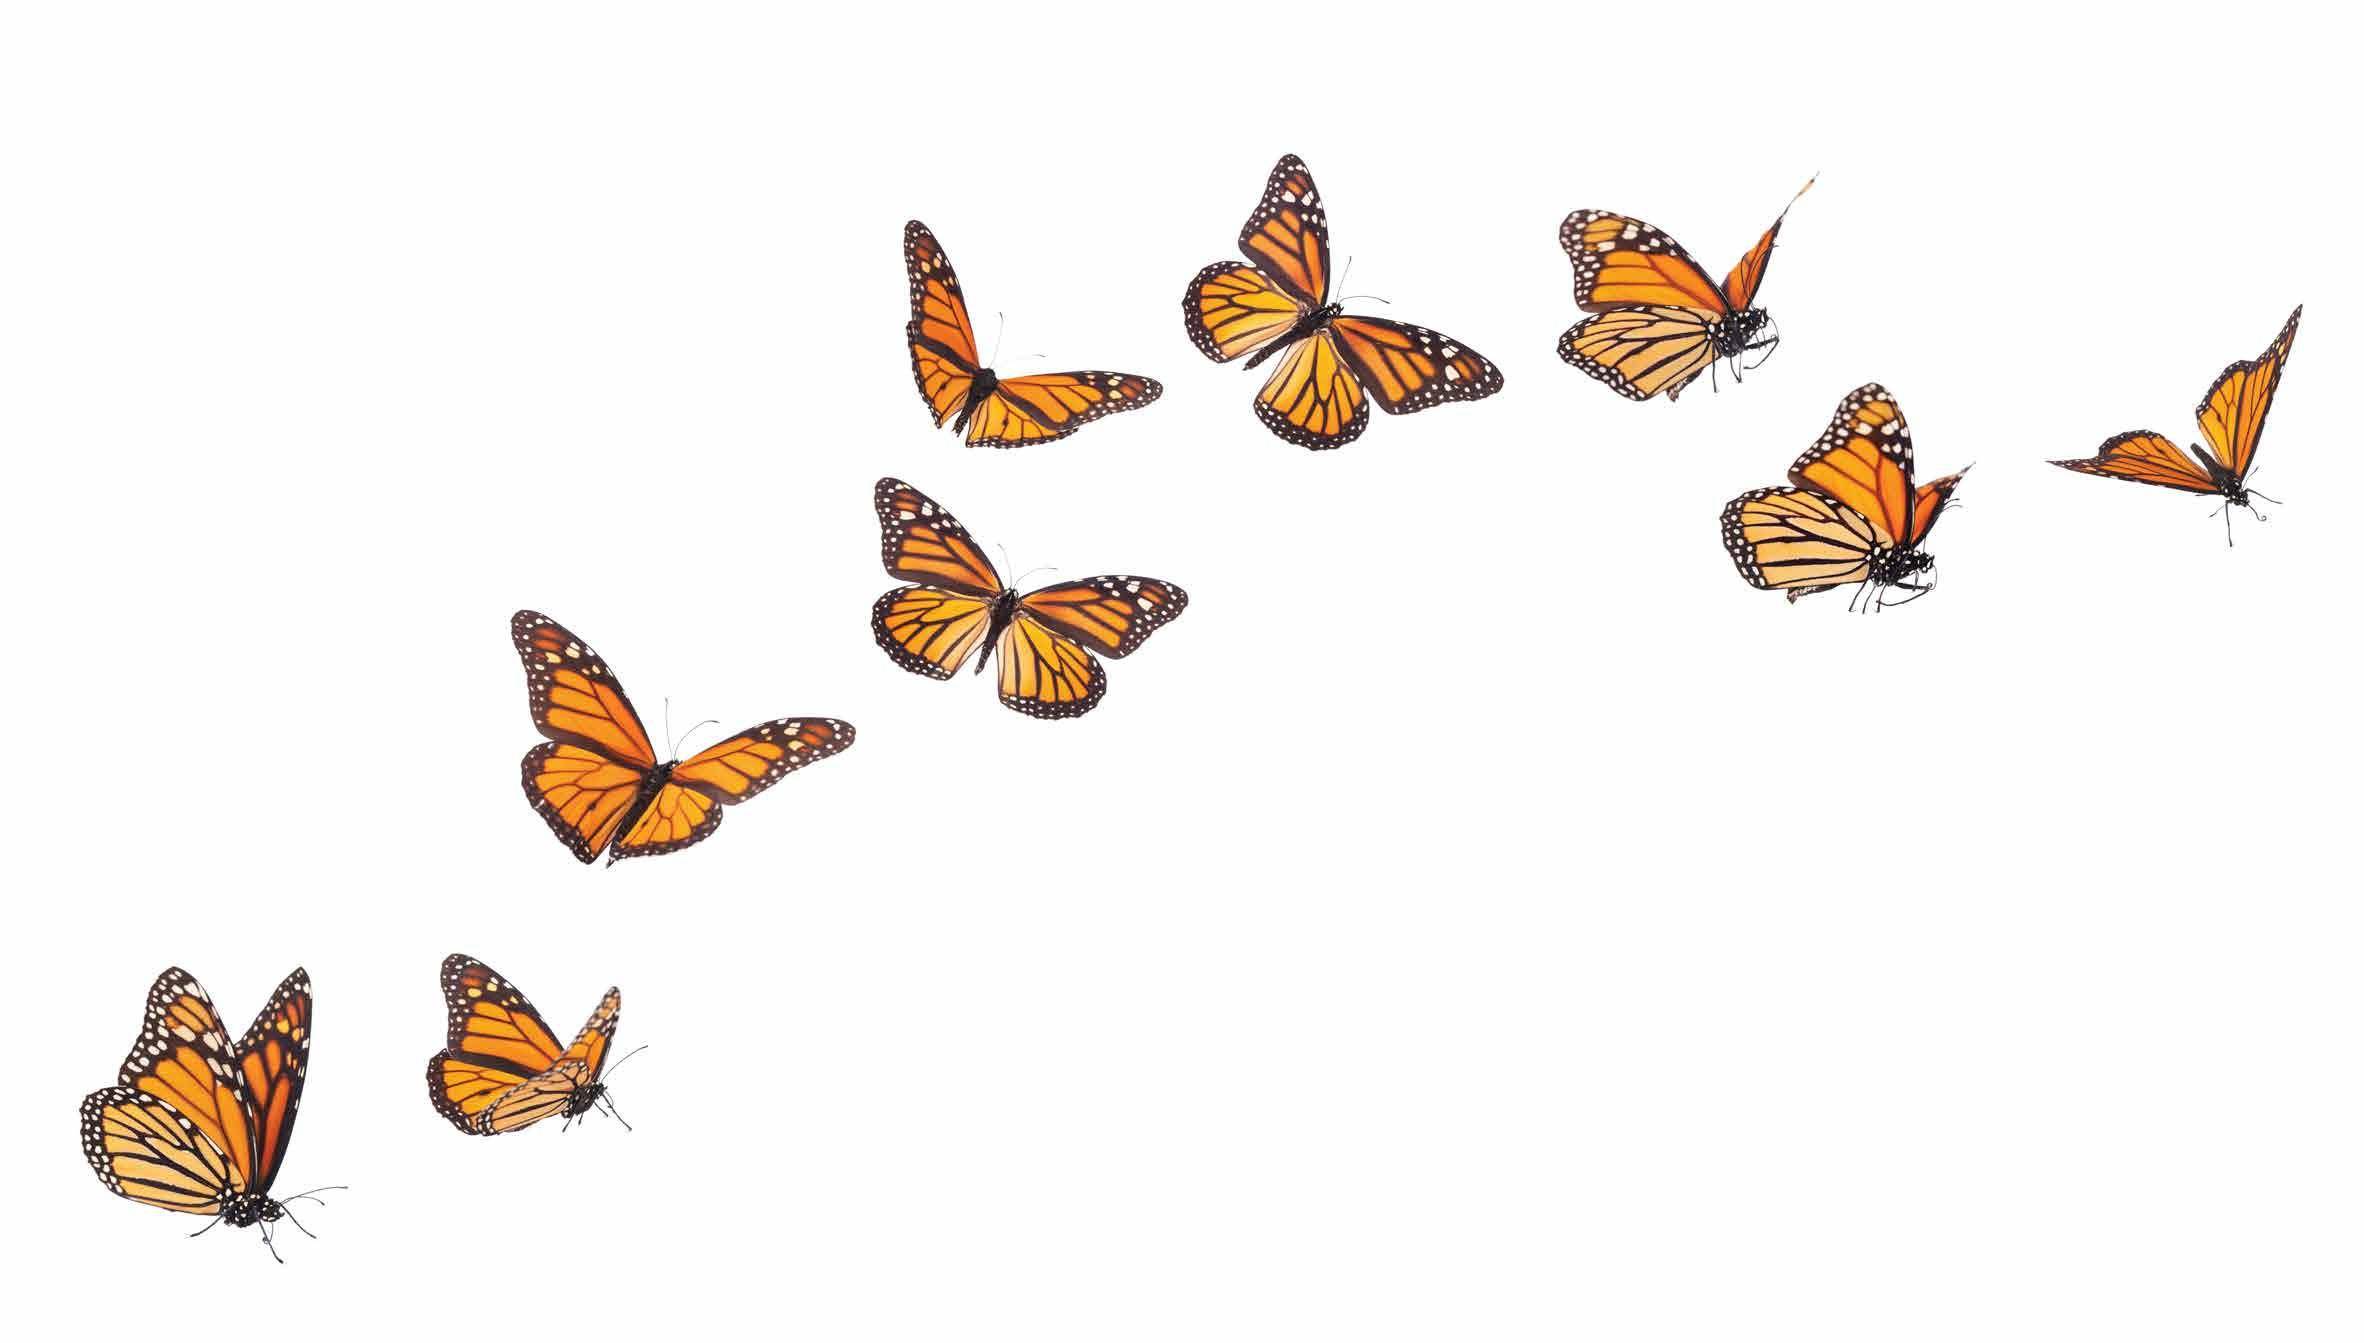
\includegraphics[width=\textwidth]{butterflies-mobile.jpg}};
}

%----------------------------------------------------------------------------------------
%	ABSTRACT
%----------------------------------------------------------------------------------------

\color{Navy} % Navy color for the abstract

\section*{Abstract}

\begin{itemize}
	\item A novel agent based, artificial life model, for the evolution of mimicry is presented.
	\item This model is a predator-prey co-evolution scenario where pattern representation phenotype is simulated with Cellular Automata (CA) \citep{Wolfram2002}, while behaviors of pattern recognition is configured with Hopfield Network.
	\item A visual three dimensional toroidal cube is used to construct a universe in which agents have complete freedom of mobility, genetic representation of behavior and reproduction capability to evolve new behaviors in successive generations \citep{grogono2003}.
	\item Agents are classified into categories of predator and prey species. Genome of prey species control their mobility and palatability, while 2D CA is used to represent a pattern, where the rule to generate the CA is also genetically represented.
	\item Using the above construction of ideas, successful emulation of the natural process of mimicry is achieved. Also complex behavior pattern of Batesian and Mullerian mimicry is simulated and studied.
\end{itemize}

%----------------------------------------------------------------------------------------
%	INTRODUCTION
%----------------------------------------------------------------------------------------

\color{SaddleBrown} 

%----------------------------------------------------------------------------------------
%	The Inspiration: Mimicry
%----------------------------------------------------------------------------------------

\section*{The Inspiration: Mimicry}
\subsection*{Batesian Mimicry}

\begin{center}\vspace{1cm}
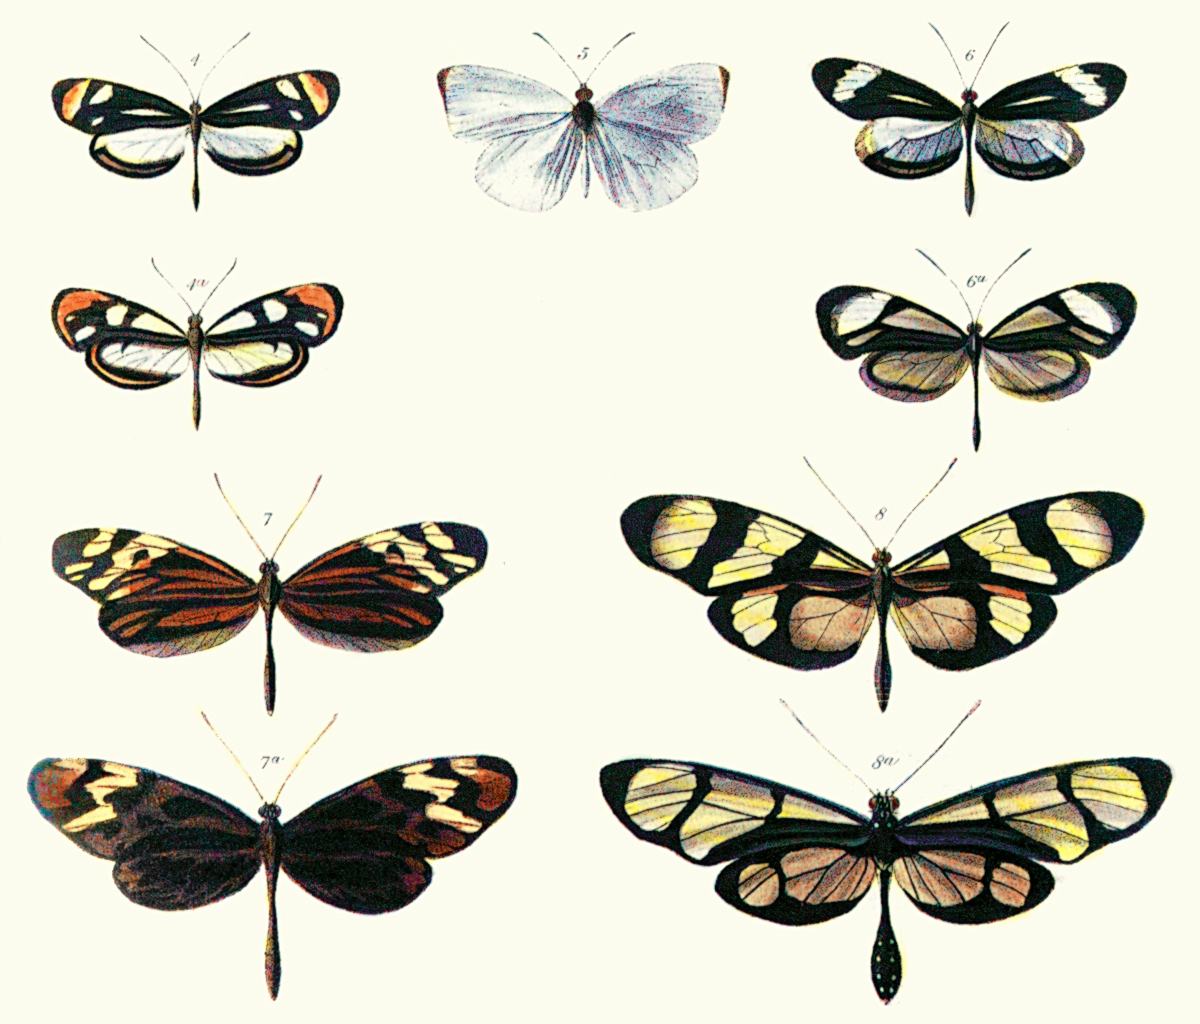
\includegraphics[width=0.5\linewidth]{Batesplate_ArM.png}
\captionof{figure}{\color{Green} Plate from Bates (1862) illustrating Batesian mimicry between Dismorphia species (top row, third row) and various Ithomiini (Nymphalidae) (second row, bottom row)}
\end{center}\vspace{1cm}

\begin{itemize}
	\item Henry W. Bates first published in 1862 his findings about the similarities and dissimilarities between Heliconiinae and Ithomiinae butterflies.
	\item He found butterflies having similar appearance, exhibiting morphological features which point to completely different species even families.
	\item Even though Heliconiids are conspicuously colored, they are extremely abundant and slow in mobility. Still predators in the surrounding area, mostly insectivorous birds do not prey on them, because of their inedible and unpalatable nature.
	\item Other edible and palatable species such as ithomiinae and pieridae, pretend to be heliconiids and thus enjoy protection.
	\item In general, the animal which is avoided by predator for unpalatable behavior is called the \textbf{model} and the imitating animal is called the \textbf{mimic}.
\end{itemize}

\color{DarkSlateGray}
\subsection*{Mullerian Mimicry}
\begin{itemize}
	\item Occasionally two inedible unrelated butterfly species are amazingly similar in appearance. An explanation for this was provided by Fritz Muller in 1878. 
	\item When there are multiple inedible species it is hard for predators to recognize each of them to know which one to consume and which one to avoid.
	\item Because of the predator's limited memory, all these species still lose their number even after being inedible. 
	\item So to save this loss, and to prevent more sacrifice of their own kind, inedible species from different families also tend to evolve to have similar appearance. 
	\item This phenomena is referred to as Mullerian Mimicry in the name of Fritz Muller. 
	\item Like Batesian mimicry, Mullerian mimicry can evolve in two stages: the mutational, one way convergence stage followed by the gradual, mutual convergence stage.
\end{itemize}

\color{SaddleBrown} 
\section*{The Model: Evolution of Mimicry}

\begin{itemize}
	\item Our model initializes with three kinds of agents. These agents have properties and behavior similar to the \textbf{model}, the \textbf{mimic} and the \textbf{predator}.
	\item We represent evolution of pattern for the model and the mimic with the help of \textbf{CA}, as \textbf{CA} can be easily represented by simple rules.
	\item Each predator is equipped with a Hopfield network, which gives it pattern recognition capability. The process of evolution occurs at the genetic level.
\end{itemize}

\begin{center}\vspace{1cm}
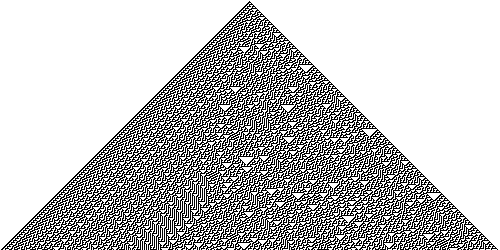
\includegraphics[width=0.50\linewidth]{CA_rule30s.png}
\captionof{figure}{\color{Green} Cellular Automata Rule 30 (Image Credit: Wikipedia)}
\label{fig:cellular-automata-rule-30}
\end{center}\vspace{1cm}

\color{DarkSlateGray}
\subsection*{The Prey: Models and Mimics}

\begin{itemize}
	\item Every prey organism contain a binary genetic representation of CA which generates a fully developed pattern of size 16 by 16 bits from its initial state.
	\item With this pattern the predator will identify the prey and store its level of palatability in memory. 
	\item We choose CA as its decimal rule can be easily represented with the help of a binary genome and evolutionary operations on the genomic representation, such as mutation and crossover can easily be applied. 
	\item To store in Hopfield memory we take a linear representation of this 2-D pattern and to find similarity between two patterns we calculate hamming distance between their linear representations.
\end{itemize}

\color{SaddleBrown} 
\subsubsection*{Reflection of punctuated equilibrium}
\label{subsubsec:reflection-of-punctuated-equilibrium}

\begin{itemize}
	\item Punctuated equilibrium is more inclined to cladogenesis instead of gradualism. Also Turner \citep{turner1988} emphasizes on punctuated equilibrium to describe the evolution of mimicry instead of phyletic gradualism. 
	\item The design of this model also follows Turner's explanation in terms of evolving mimicry.
	\item New CA patterns evolve from existing ones in prey population just by a single mutation in the pattern gene. 
\end{itemize}

\begin{center}\vspace{1cm}
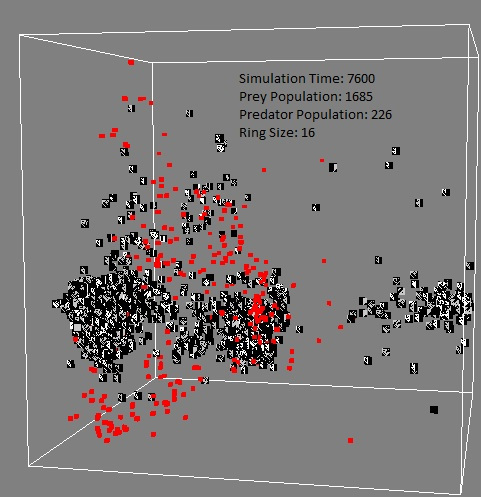
\includegraphics[width=0.5\linewidth]{simTime7600.png}
\captionof{figure}{\color{Green} Graphical representation of the model, simulation time: 7600}
\end{center}\vspace{1cm}

\color{SaddleBrown} 
\subsection*{Predator}

\begin{itemize}
	\item Predators in the system are designed to provide selection pressure to \textit{models} and \textit{mimics} for the evolution of mimicry. 
	\item These agents are equipped with Hopfield Network Memory to be able to learn and recognize patterns of the prey species.
	\item Their mobility and reproduction capability are controlled at the genetic level, while their memory is not genetically controlled, as we could not find a suitable encoding for the genetic representation of Hopfield Network.
	\item Every new predator is born with zero memory and with no inheritance from parents.
\end{itemize}

\color{DarkSlateGray}
\subsubsection*{Learning}

\begin{itemize}
	\item The objective of a predator's interaction with prey is always to consume it. But based on the prey's pattern and palatability, the predator will either be able to consume it or throw it back to the environment. 
	\item At this event the predator needs to learn the pattern with which the prey has been represented. The pattern represents palatability of the prey species, at least to the predator. 
	\item Every time a new interaction is made by the predator its memory is initialized with all the existing pattern that has already been encountered and the new one.
	\item The learning procedure used for this memory is Hebbian Learning \citep{hebb1949}, which represents a purely feed-forward, unsupervised learning. 
\end{itemize}

\color{DarkSlateGray}
\section*{The Results}

\begin{itemize}
	\item Data and analysis in this simulation has been concentrated on evaluating whether evolution of mimicry has taken place.
	\item This evaluation can be made with the number of different rings that has been created and the size of each of those rings along with the population of palatable and unpalatable species.
	\item Also it can be established whether Batesian Mimicry and Mullerian Mimicry have taken effect by analyzing the data set of these populations.
\end{itemize}

\begin{center}\vspace{1cm}
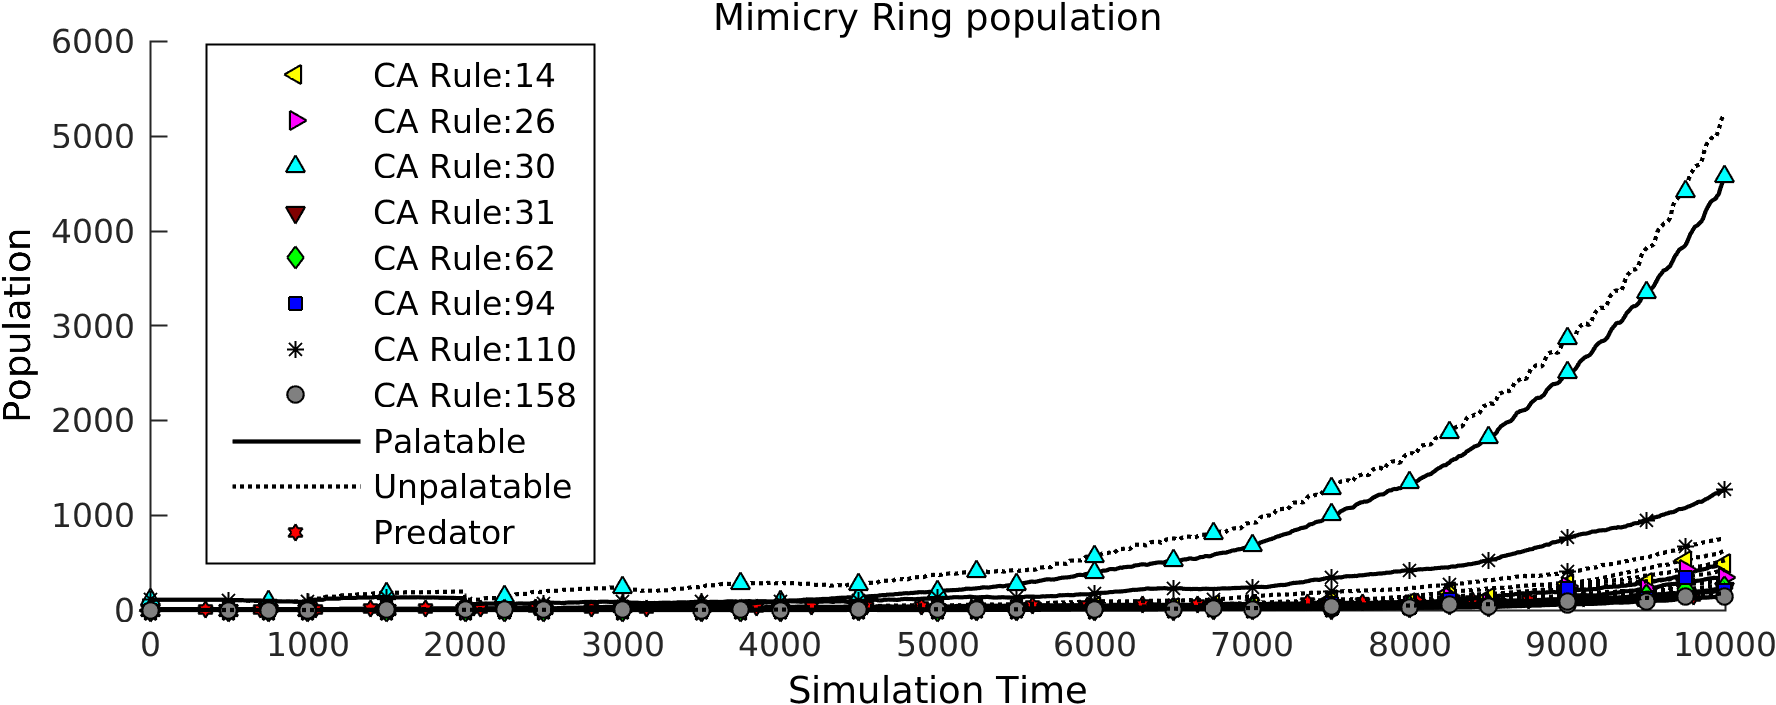
\includegraphics[width=0.8\linewidth]{simTime10k-2Prey.png}
\captionof{figure}{\color{Green} Population distribution of mimicry rings, initialized with 2 prey species, 10k iterations}
\label{fig:2prey-species}
\end{center}\vspace{1cm}

\color{SaddleBrown} 
\subsection*{Analysis}
\begin{itemize}
\item Batesian mimicry has taken effect as it can be observed (figure \ref{fig:2prey-species}) that for every ring of unpalatable species there is an existence of the palatable ring racing to reach the population count of its unpalatable counterpart.
\item Effects of Mullerian mimicry can also be observed best for the experiment initialized with only unpalatable prey species (figure \ref{fig:unpalatable-species}). We initialized the model with 4 rings of unpalatable species with no palatable ones and after nearly 10K iterations, all of the initial unpalatable rings have survived with dominance. 
\end{itemize}

\begin{center}\vspace{1cm}
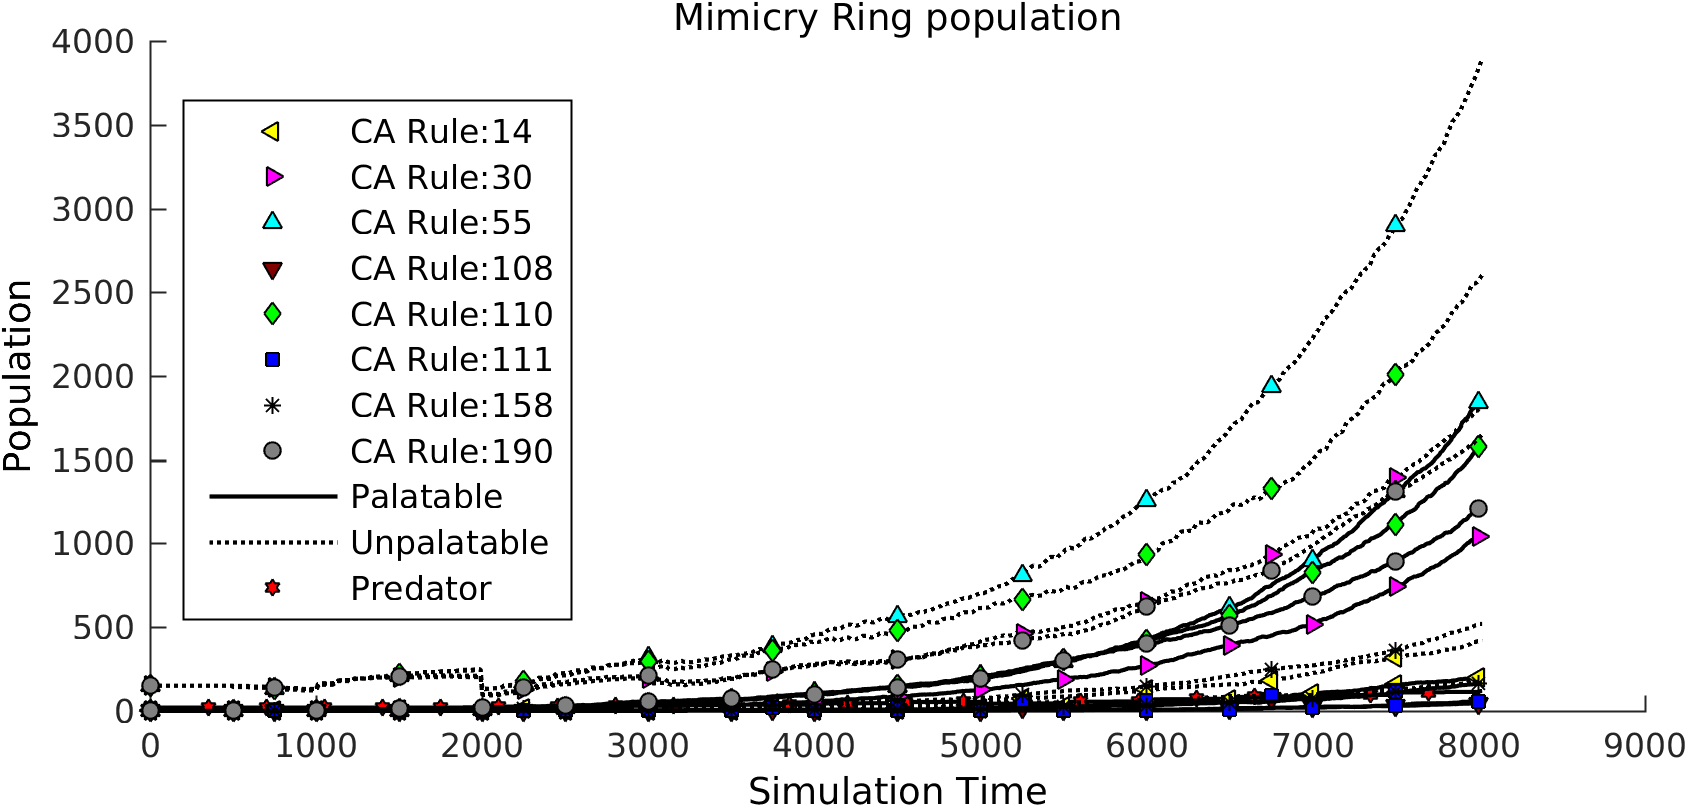
\includegraphics[width=0.8\linewidth]{simTime8k-4Prey-unp.png}
\captionof{figure}{\color{Green} Population distribution of mimicry rings, initialized with 4 prey species all unpalatable}
\label{fig:unpalatable-species}
\end{center}\vspace{1cm}

%----------------------------------------------------------------------------------------
%	CONCLUSIONS
%----------------------------------------------------------------------------------------
\color{DarkSlateGray}
\section*{Conclusions}
\begin{itemize}
\item Analysis of the results tell us that we have successfully been able to simulate the evolution of mimicry.
\item This model provides a more accurate simulation of the fascinating natural process of mimicry rings and their shift in population. 
\item This model also verifies the theory of Turner in explaining the evolution of mimicry with punctuated equilibrium.
\end{itemize}

 % Set the color back to DarkSlateGray for the rest of the content

%----------------------------------------------------------------------------------------
%	REFERENCES
%----------------------------------------------------------------------------------------
\color{SaddleBrown} 
%\nocite{*} % Print all references regardless of whether they were cited in the poster or not
\bibliographystyle{plain} % Plain referencing style
\bibliography{references} % Use the example bibliography file sample.bib

%----------------------------------------------------------------------------------------

\end{multicols}
\end{document}